\documentclass{article}
\usepackage{listings}
\usepackage{mathrsfs}
\usepackage[utf8]{inputenc}
\usepackage{amssymb}
\usepackage{lipsum}
\usepackage{amsmath}
\usepackage{fancyhdr}
\usepackage{geometry}
\usepackage{scrextend}
\usepackage[english,german]{babel}
\usepackage{titling}
\setlength{\droptitle}{-3cm}
\usepackage{tikz}
\usepackage{algorithm,algpseudocode}
\usepackage[doublespacing]{setspace}
\usetikzlibrary{datavisualization}
\usetikzlibrary{datavisualization.formats.functions}
\usepackage{polynom}
\usepackage{amsmath}
\usepackage{gauss}
\usepackage{tkz-euclide}
\usetikzlibrary{datavisualization}
\usetikzlibrary{datavisualization.formats.functions}
\author{
Alexander Mattick Kennung: qi69dube\\
Kapitel 1
}
\usepackage{import}
\date{\today}
\geometry{a4paper, margin=2cm}
\usepackage{stackengine}
\parskip 1em
\newcommand\stackequal[2]{%
  \mathrel{\stackunder[2pt]{\stackon[4pt]{=}{$\scriptscriptstyle#1$}}{%
  $\scriptscriptstyle#2$}}
 }
\makeatletter
\renewcommand*\env@matrix[1][*\c@MaxMatrixCols c]{%
  \hskip -\arraycolsep
  \let\@ifnextchar\new@ifnextchar
  \array{#1}}
\makeatother
\lstset{
  language=haskell,
}
\lstnewenvironment{code}{\lstset{language=Haskell,basicstyle=\small}}{}
\usepackage{enumitem}
\setlist{nosep}
\usepackage{titlesec}

\titlespacing*{\subsection}{0pt}{2pt}{3pt}
\titlespacing*{\section}{0pt}{0pt}{5pt}
\titlespacing*{\subsubsection}{0pt}{1pt}{2pt}
\title{Vorlesung 4}


\begin{document}
	\maketitle
	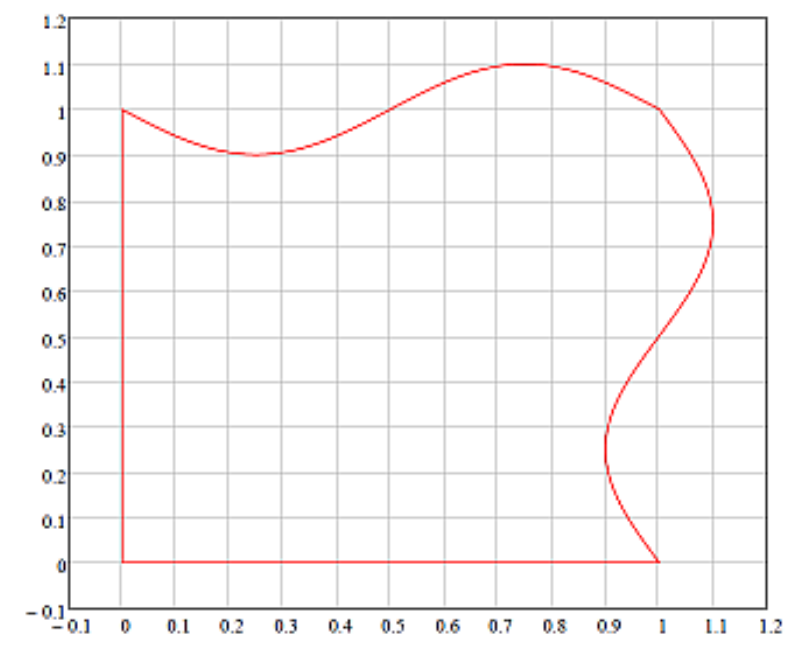
\includegraphics[width=256px]{Menge.png}\\
	$\underline{y}(x)\leq \bar y(x) \forall x\in [a,b]$\\
	$G=\{(x,y)\in\mathbb{R}^2|x\in[a,b], \underline{y}(x)\leq y\leq \bar y(x)\}$\\
	$G=\{(x,y)\in\mathbb{R}^2|y\in[a,b], \underline{x}(x)\leq x\leq \bar x(x)\}$\\
	$G_y:=\{(x,y)\in\mathbb{R}^2|x\in[0,1],x\leq y\leq 1-\frac{1}{10}\sin(2\pi x)\}$
	und\\
	$G_x:=\{(x,y)\in\mathbb{R}^2| y\in[0,1], y\leq x\leq 1-\frac{1}{10}\sin(2\pi x)\}$\\
	Die periode des sinus erhält man durch strecken der sinusfunktion, und wir haben einen offset von +1 nach oben. Außerdem fällt die sinusfunktion zuerst, also $-\sin(2\pi x)+1$.\\
	$G=\{x\in\mathbb{R}^2: ||x||\leq 2\}$ und $f(x)=1+x_1^2+x_2^2$\\
	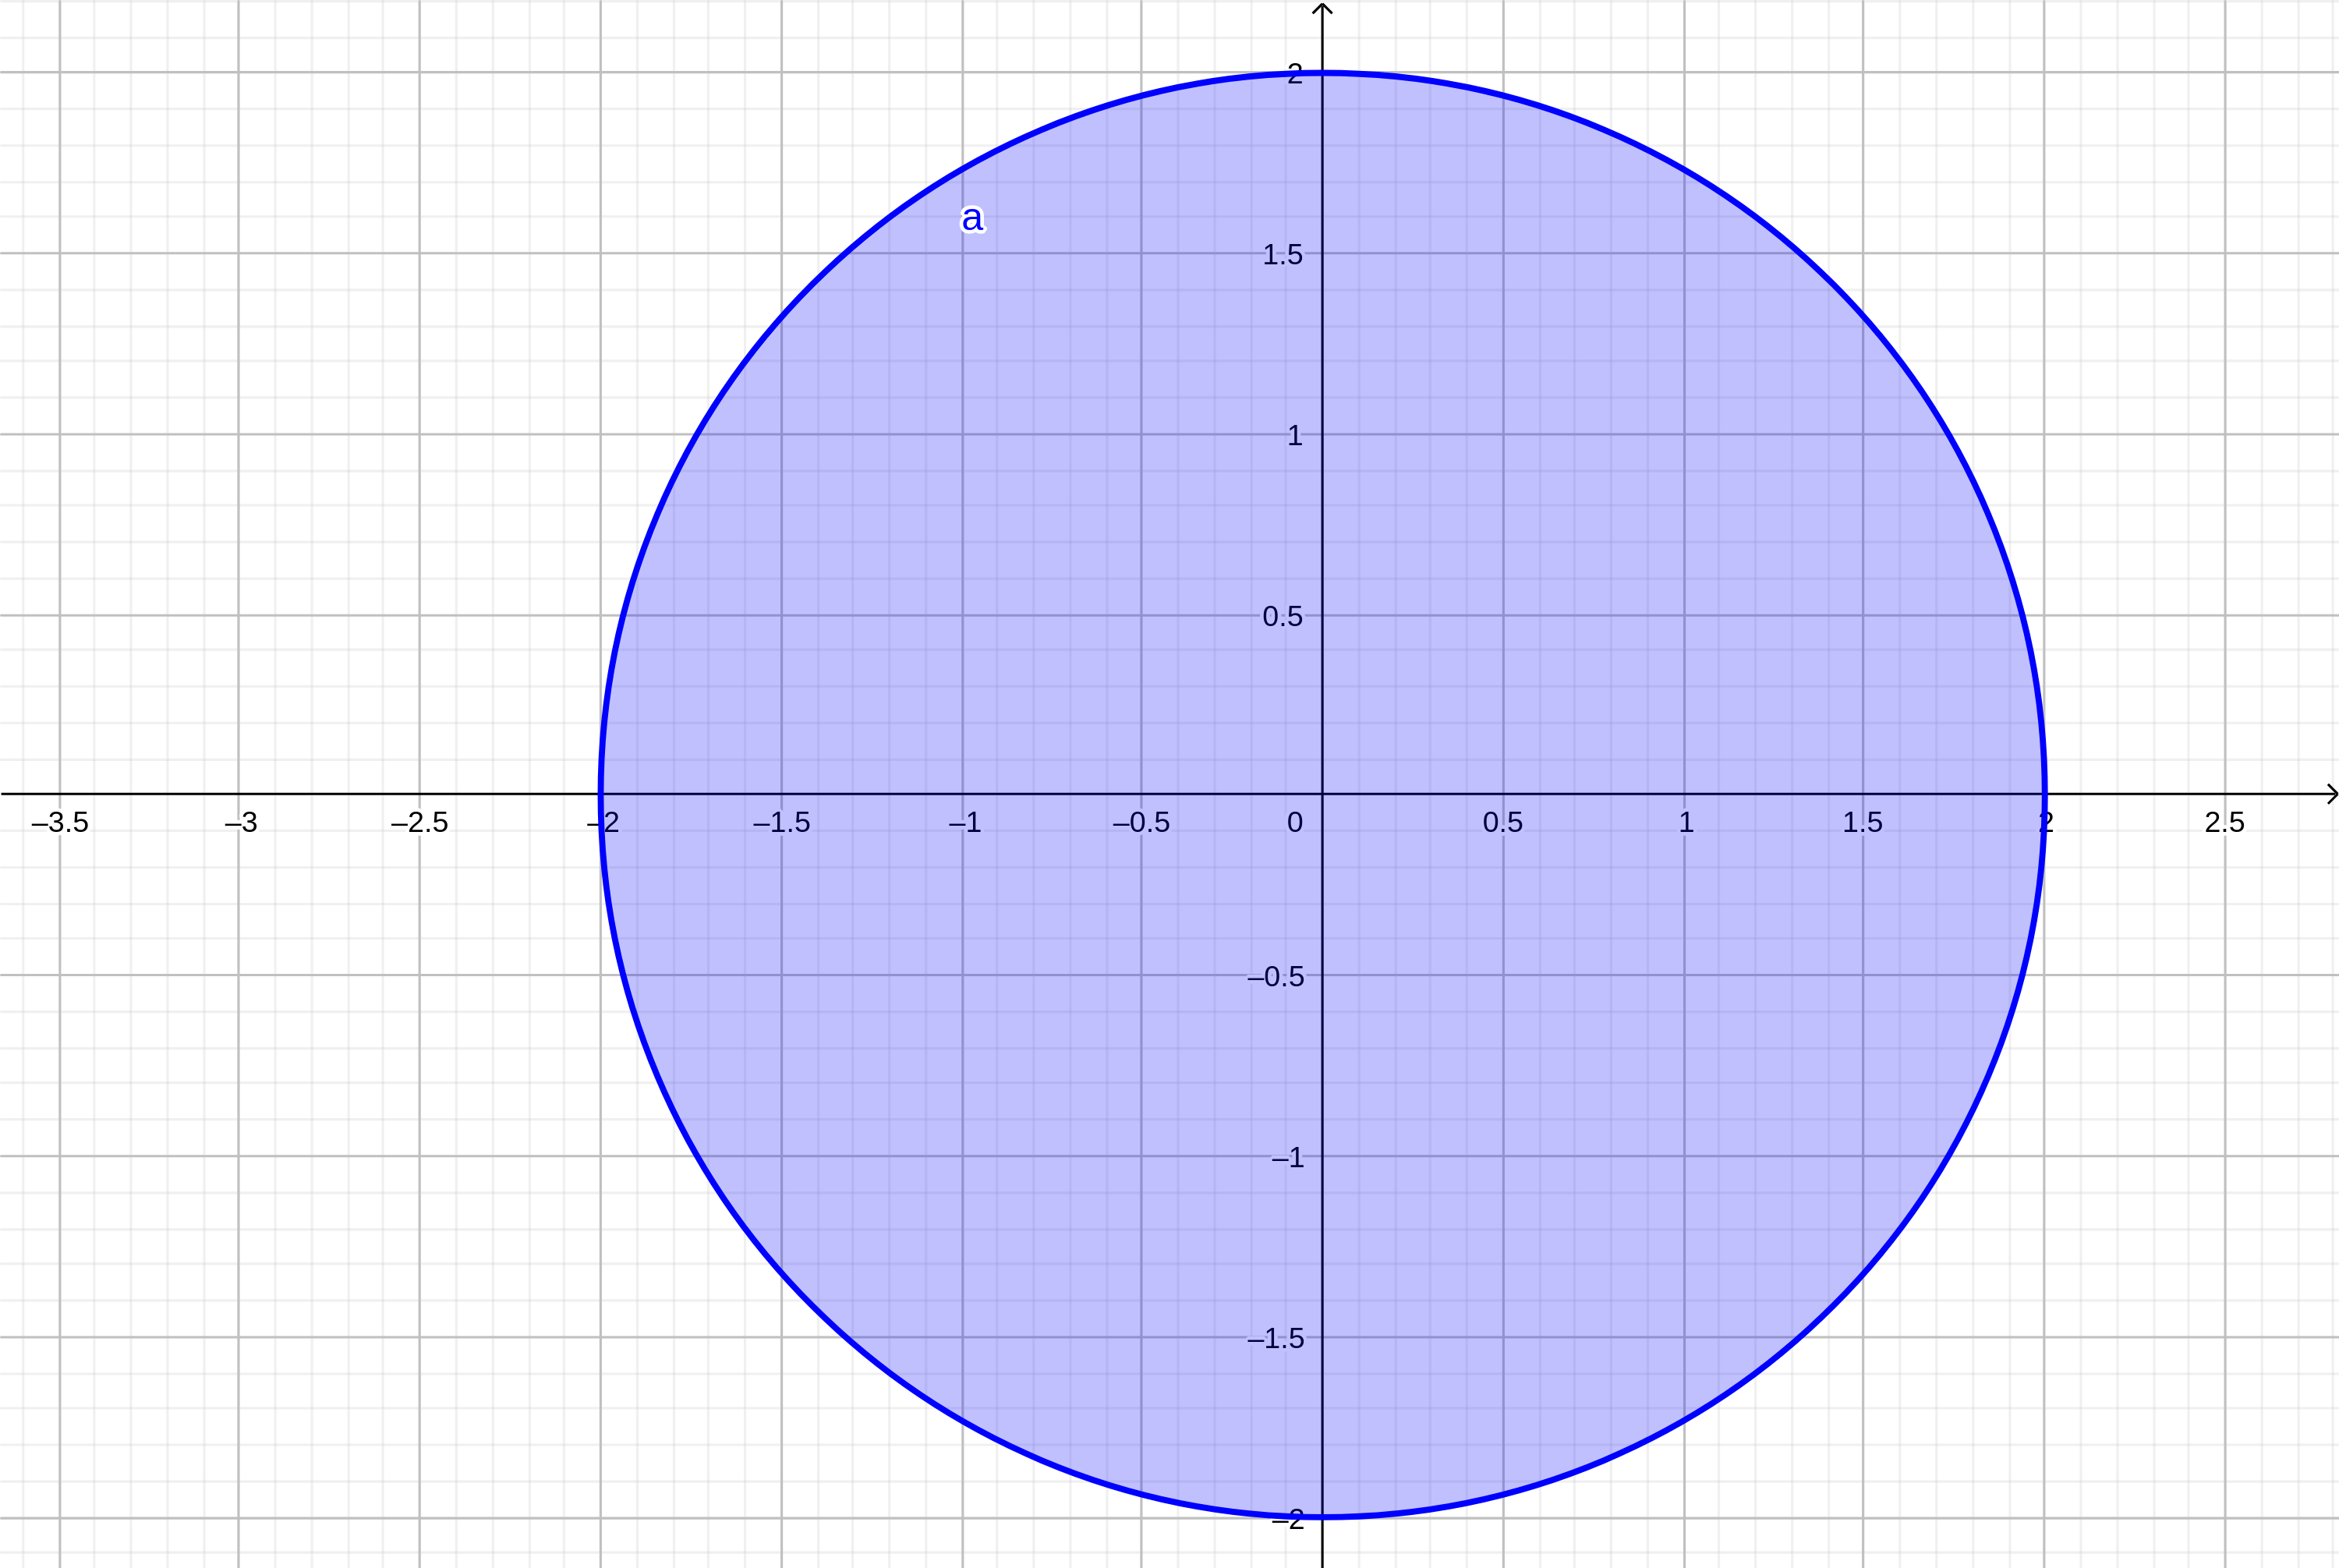
\includegraphics[width=256px]{KreisG.png}\\
	$$\int_G f(x,y)dxdy = \int_\alpha^\beta \int^{h_2(\theta)}_{h_1(\theta)} f(r\cos(\theta),r\sin(\theta))rdrd\theta$$
	\textbf{(also transformation in Polarkoordinaten ist wichtig)\\}
	$t(r,\theta)= (r\cos(\theta),r\sin(\theta))$ (t muss bijektiv, stetig diff'bar sein, wobei das inverse auch stetig diffbar sein muss: Diffeomorphismus)\\
	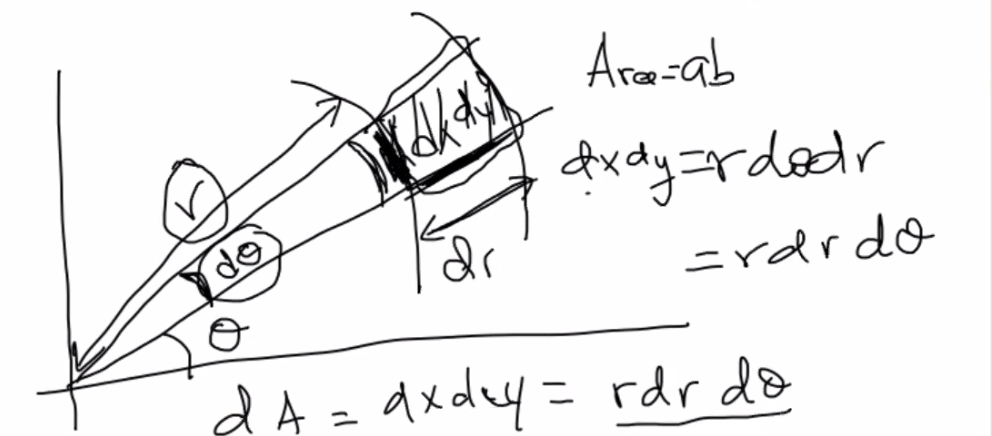
\includegraphics[width=256px]{GeometrischeInterpretation.png}
	Der Grund, warum das *r am ende hinzukommt ist, dass man die differentialfläche  hinzufügen muss $A = dx*dy = r* dr*d\theta$\\
	Also wir bekommen $\bar G = \{x\in\mathbb{R}^2: 0\leq r\leq 2, 0\leq \theta\leq 2\pi\}$\\
	$f(x,y)=1+x^2+y^2$\\
	nach transformation also $f(r\cos(\theta),r\sin(\theta)) = 1+r^2\cos^2(\theta)+r^2\sin^2(\theta) = 1+r^2$\\
	$$\int_G(1+x^2+y^2)dxdy = \int^2_0\int ^{2\pi}_0 (1+r^2)rd\theta dr$$
	$$\int_0^2 2\pi (r+r^3)dr$$
	$$2\pi\int_0^2  (r+r^3)dr$$
	$$2\pi[(\frac{1}{2}r^2+\frac{1}{4}r^4)]^2_0$$
	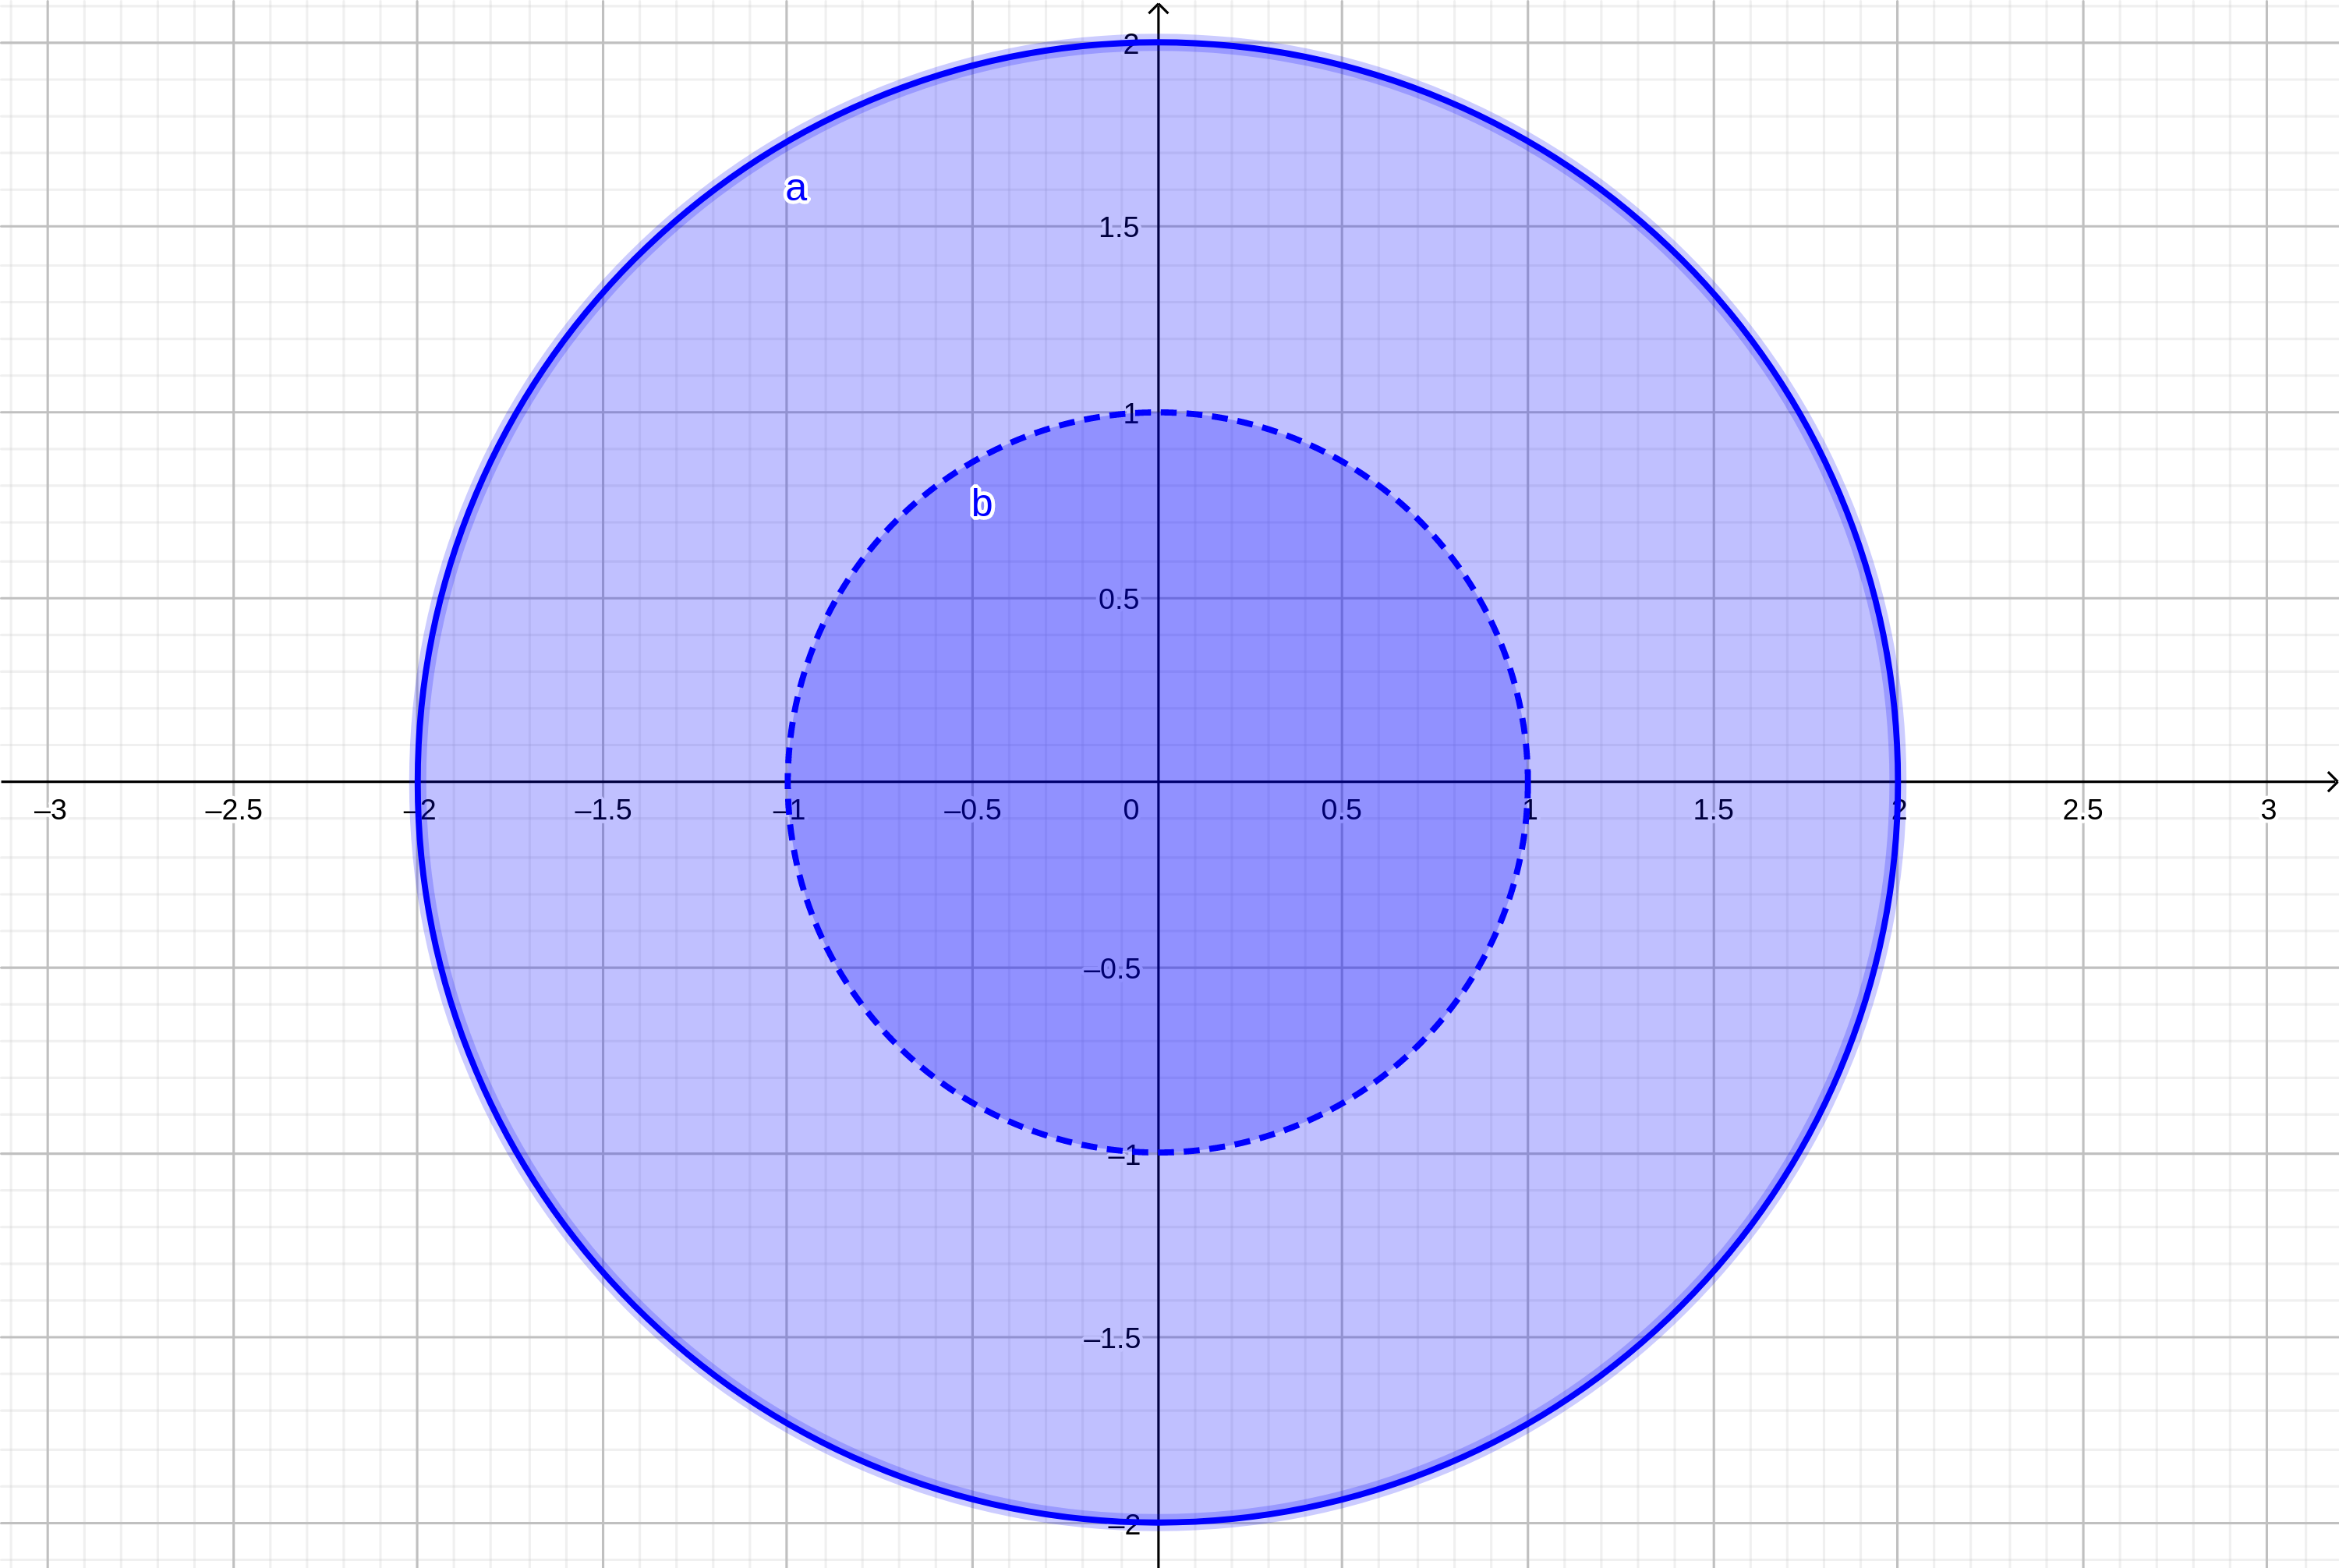
\includegraphics[width=256px]{2Beispiel.png}
	Wenn man über die Fläche zwischen den beiden Kreisen integrieren möchte, dann geht man über die Fläche:\\
	$G=\{(r,\theta)\in\mathbb{R}^2|1\leq r\leq 2, 0\leq \theta\leq 2\pi\}$\\
	Wenn man nur über die obere Fläche integrieren möchte:\\
	$$G=\{(r,\theta)\in\mathbb{R}^2|1\leq r\leq 2, 0\leq \theta\leq 1\pi\}$$
\end{document}